%\appendix
\begin{landscape}
\section{APPENDIX B} \label{sec:appB}

\subsection*{B1 Air Sampling Control Object Sequence diagrams}
\begin{figure}[H]
    \centering
    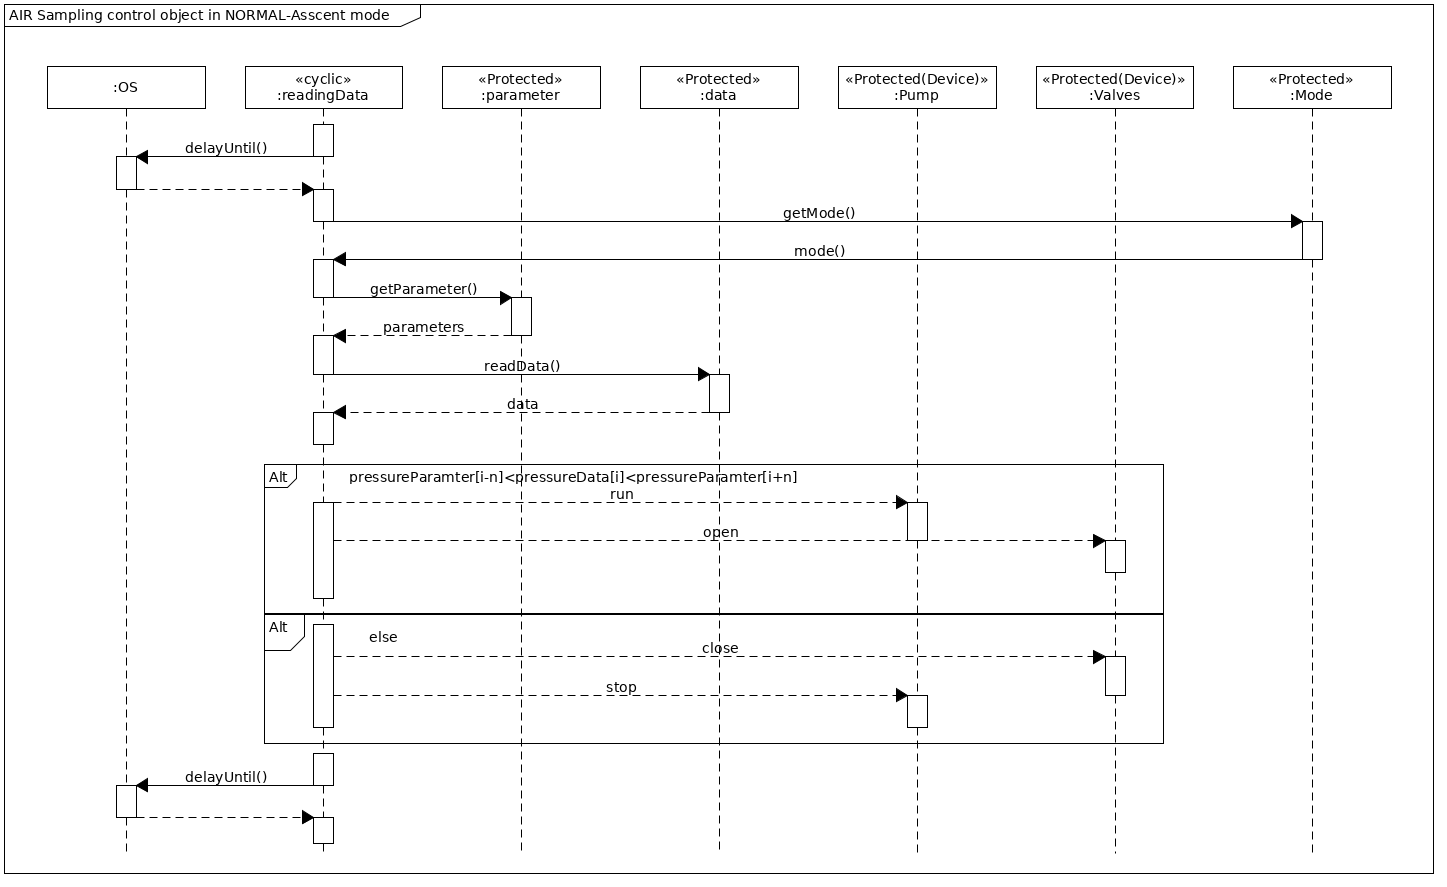
\includegraphics[height=0.75\textwidth]{appendix/img/ASC-seq-dia-v1-2-a.png}
    \caption{ASC object in normal mode -Ascent.}
    \label{ASCa}
\end{figure}

\begin{figure}[H]
    \centering
    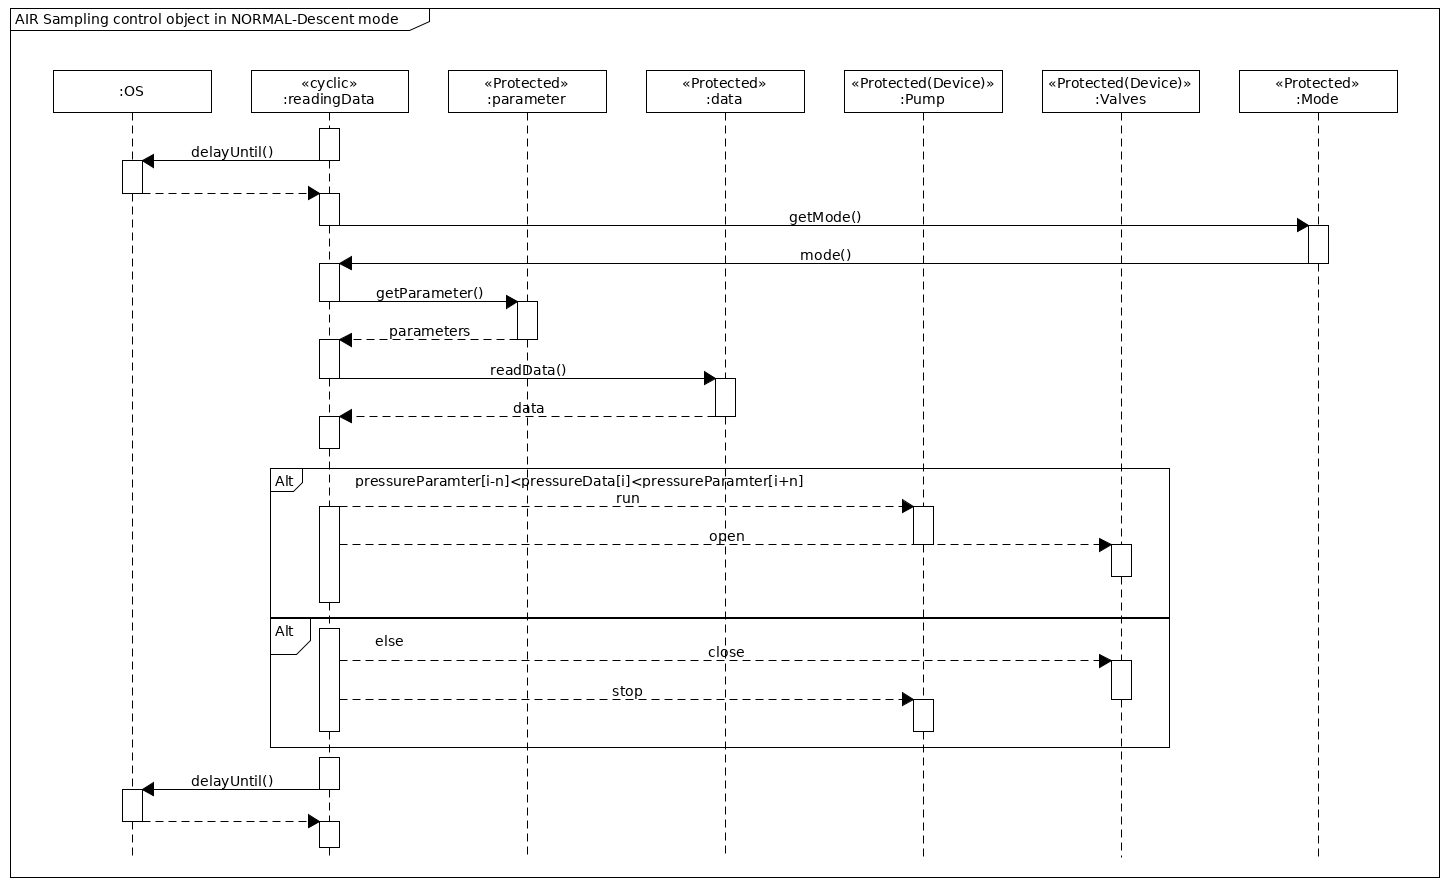
\includegraphics[height=0.9\textwidth]{appendix/img/ASC-seq-dia-v1-2-b.png}
    \caption{ASC object in normal mode -Descent.}
    \label{ASCb}
\end{figure}
\begin{figure}[H]
    \centering
    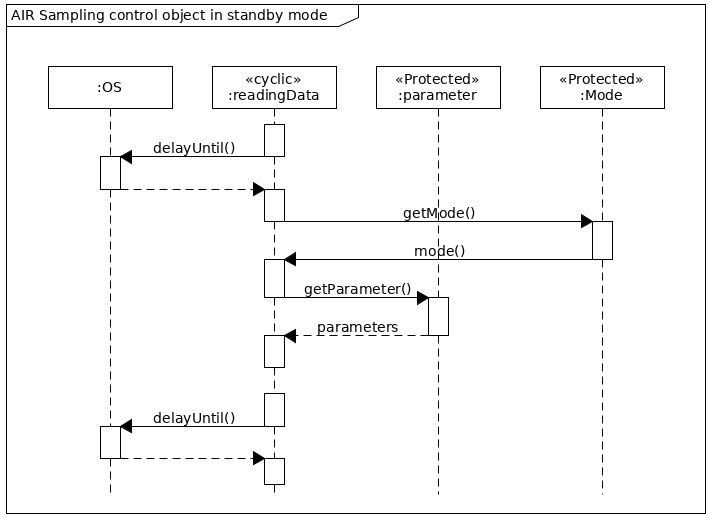
\includegraphics[height=0.9\textwidth]{appendix/img/ASC-seq-dia-v1-2-c.png}
    \caption{ASC object in standby mode.}
    \label{ASCb}
\end{figure}
\subsection*{B2 Heating Object Sequence Diagrams}
\begin{figure}[H]
    \centering
    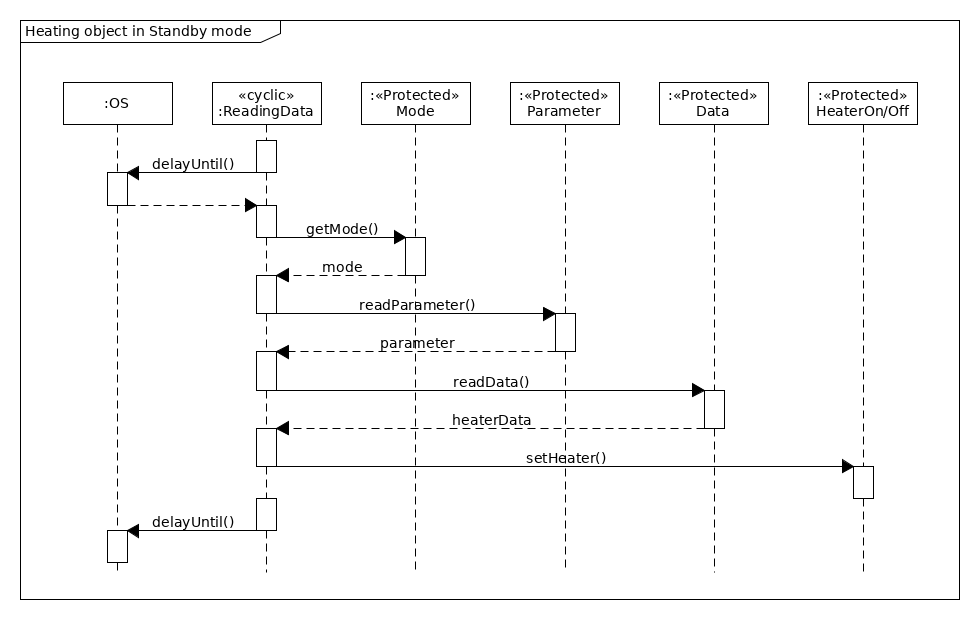
\includegraphics[height=0.9\textwidth]{appendix/img/heater-seq-dia-a.png}
    \caption{Heating object in standby mode.}
    \label{heatera}
\end{figure}
\begin{figure}[H]
    \centering
    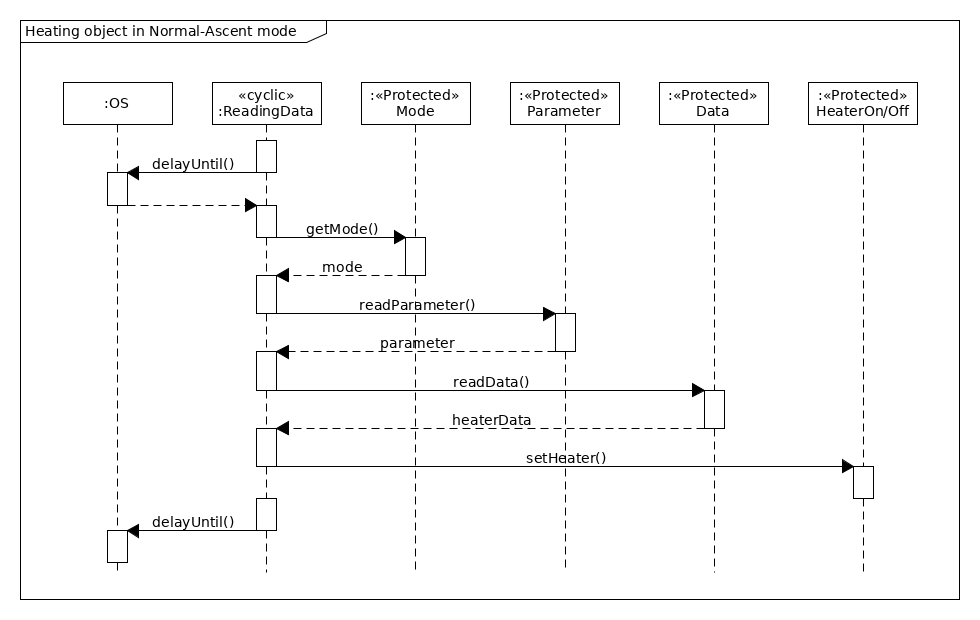
\includegraphics[height=0.9\textwidth]{appendix/img/heater-seq-dia-b.png}
    \caption{Heating object in normal mode -Ascent.}
    \label{heaterb}
\end{figure}
\begin{figure}[H]
    \centering
    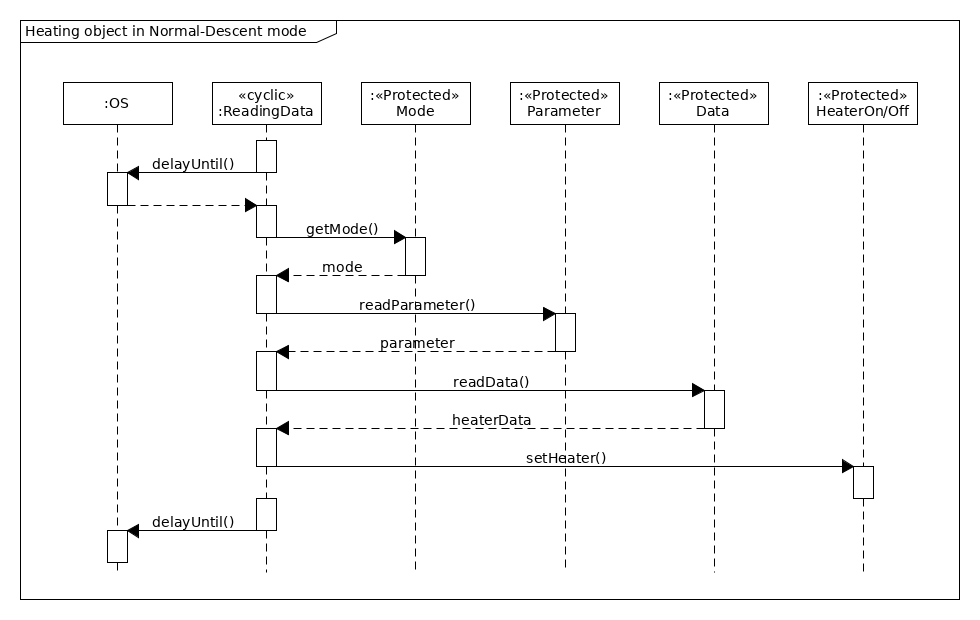
\includegraphics[height=0.9\textwidth]{appendix/img/heater-seq-dia-c.png}
    \caption{Heating object in normal mode -Descent.}
    \label{heaterc}
\end{figure}
\subsection*{B3 Sensor Object Sequence Diagrams}
\begin{figure}[H]
    \centering
    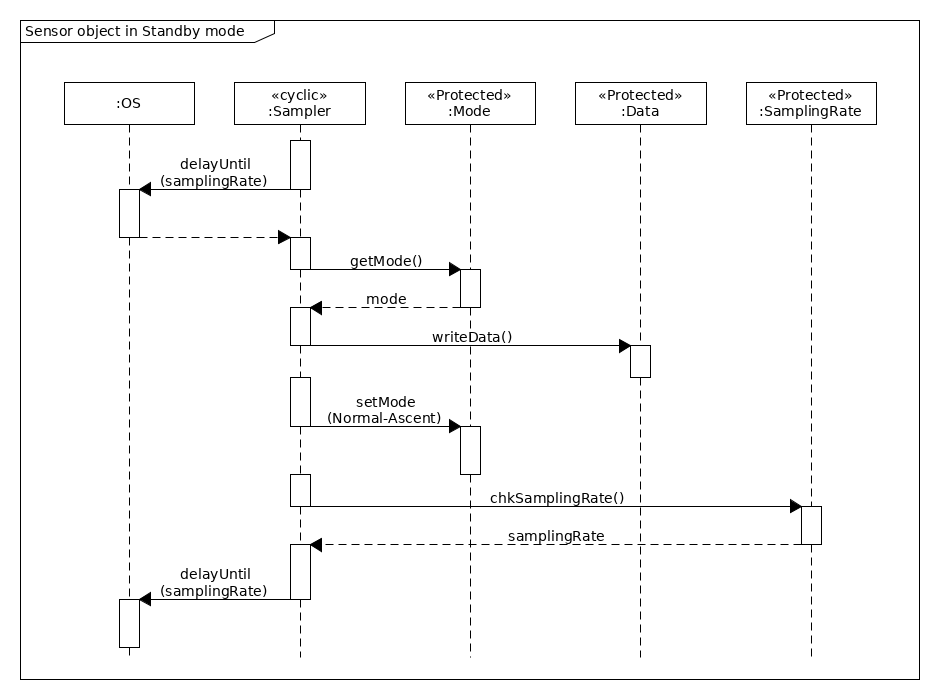
\includegraphics[height=0.9\textwidth]{appendix/img/sensor-seq-dia-a.png}
    \caption{Sensor object in standby mode}
    \label{sensora}
\end{figure}
\begin{figure}[H]
    \centering
    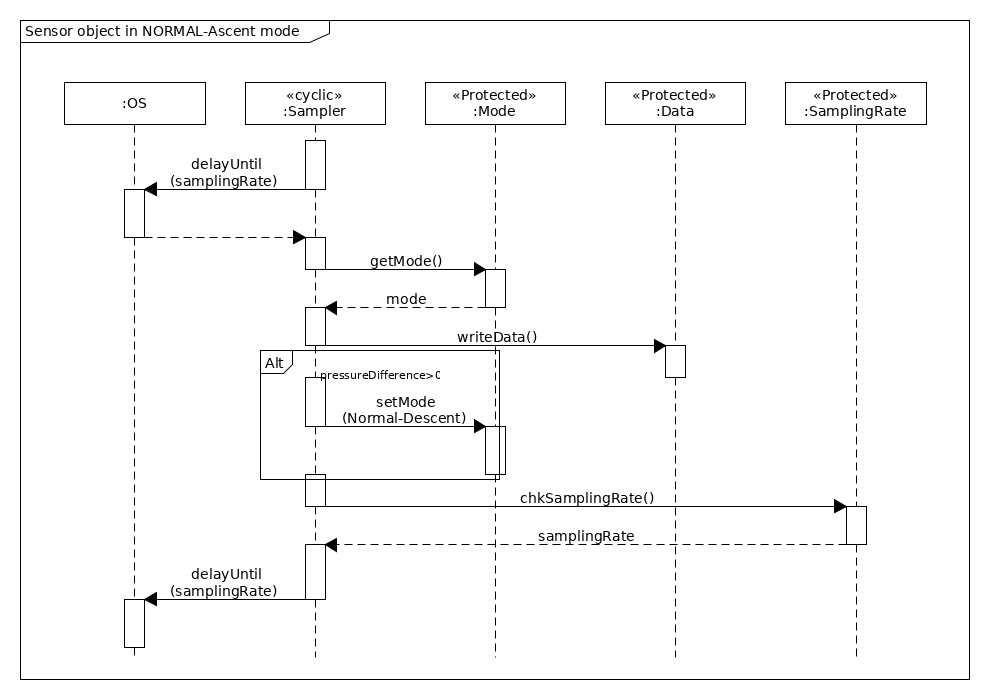
\includegraphics[height=0.9\textwidth]{appendix/img/sensor-seq-dia-b.png}
    \caption{Sensor object in normal -Ascent mode}
    \label{sensorb}
\end{figure}
\begin{figure}[H]
    \centering
    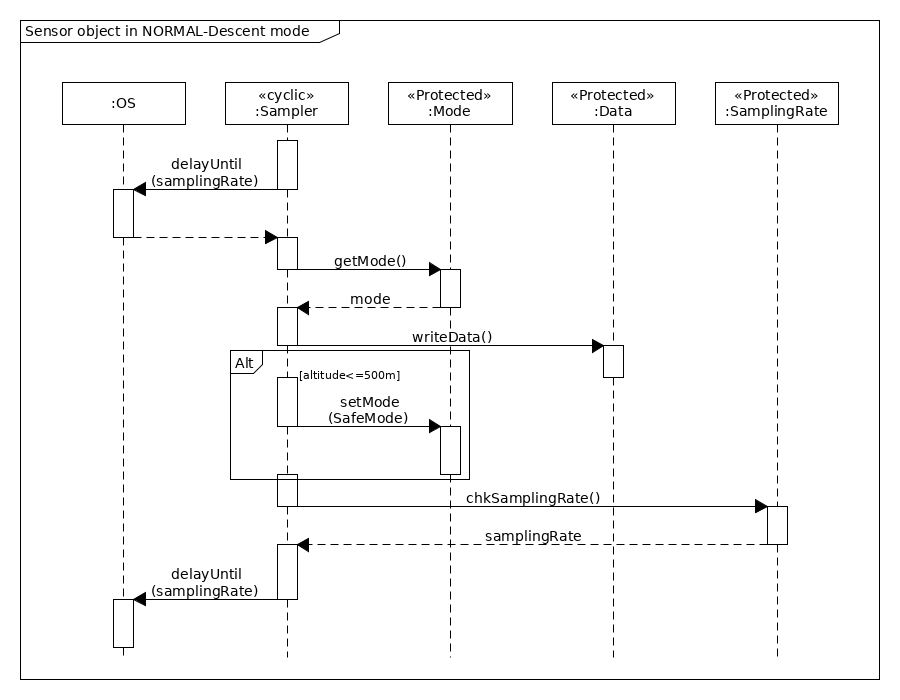
\includegraphics[height=0.9\textwidth]{appendix/img/sensor-dia-seq-c.png}
    \caption{Sensor object in normal -Descent mode}
    \label{sensorc}
\end{figure}
\end{landscape}